% PAVEL E. DOLGIREV
 
 
 
  Consider an ellipse $\E$ given by $x^2/a^2+y^2/b^2=1$ with foci $F_1=[-c,0],\; F_2=[c,0]$ and centered at $0=[0,0].$
  
  Referring to \cref{fig:pics-09- polar-ellipse}
  
  \begin{figure}
      \centering
      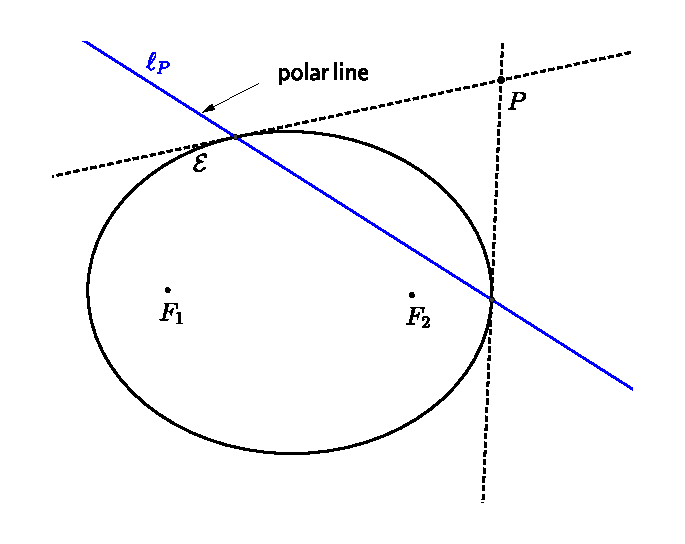
\includegraphics[scale=0.7]{pics_09_010_polarline-elipse.pdf}
      \caption{Polar line $\ell_P$.}
      \label{fig:pics-09- polar-ellipse}
  \end{figure}
 \begin{definition}
The polar of a point $P$ with respect to $\E$ is a line $\ell_{P}$ passing through the intersection points  of the two tangent lines to the ellipse passing through $P_0$.
 \label{def:09-polarline}
 \end{definition}
 
 \begin{lemma}
 The polar line   of a point $P_0=(x_0,y_0)\ne 0$ with respect to  $\E$  is given by
 %\[ b^2x_0 x+a^2 y_0y-a^2b^2=0.\]
 \begin{align}
\ell_{P_0}: \;\; \frac{x_0x}{a^2}+\frac{y_0y}{b^2}-1=0 \label{eqn:09-polarline}
\end{align}
  \label{lem:09-polarline}
  \end{lemma}
  
  \begin{proof}
  The pair of tangent lines to $\E$ passing through the point $P_0=(x_0,y_0)$ is given by
 \[ \left( x{ y_0}-y{x_0} \right) ^{2}-{b}^{2} \left( x-{  x_0}
 \right) ^{2}-{a}^{2} \left( y-{ y_0} \right) ^{2}=0 \]
 Computing the intersection with the ellipse we obtain the points $P_1$ and $P_2$ given by:
 \begin{align*}
     P_1 &= \left[\frac{ a^2\left(b^2 x_0 +   y_0\sqrt{g_0-a^2b^2}\right)}{g_0},   \frac{b^2\left(a^2y_0 -  x_0\sqrt{g_0-a^2b^2}\right)}{g_0} \right] \\
      P_2 &= \left[\frac{ a^2\left(b^2 x_0 -   y_0\sqrt{g_0-a^2b^2}\right)}{g_0},   \frac{b^2\left(a^2y_0+  x_0\sqrt{g_0-a^2b^2}\right)}{g_0} \right] 
 \end{align*}
 where $g_0=b^2x_0^2+a^2y_0^2.$
 It is straightforward do obtain that the polar line is that given by  \cref{eqn:09-polarline} which passes through  $P_1$ and $P_2$.
  \end{proof}
  
  \begin{remark} When $P_0$ is interior to $\E$ the intersections obtained above are complex.
  In this case consider two lines $\ell_1$ and $\ell_2$ passing through $P_0$. Let $Q_{1,i} $ and $Q_{2,i} $ be the intersections of $\ell_i$ with $\E$. The   tangent lines to $\E$ passing though these points determine a point $P_i$ exterior to $\E$. The line passing through $P_1$ and $P_2$ is the polar of $P_0$ with respect to $\E.$  
  \end{remark}
\begin{definition}
The pole of a line $\ell$ not passing through $0$ (center of $\E$) with respect to $\E$ is the point of  intersection of the two tangent lines passing through  $\ell\cap\E={P_1,P_2}$.
\label{def:09-pole}
\end{definition}

\begin{lemma} If the line $\ell$ is given by $x_0 x /a^2+y_0y/b^2=1$, then the pole is $[x_0,y_0].$
\label{lem:09-polar}.
\end{lemma}
\begin{proof}
Left to the reader.
\end{proof}

\begin{example} The pole of the line $2x+y-10=0$ with respect to the ellipse $x^2/3+y^2/4=1$ is the point
$[3/5,2/5]$.
\label{exa:09-pole}
\end{example}

\begin{remark}
When $\ell\cap\E=\emptyset $ to determine the pole of $\ell$ (as in   \cref{exa:09-pole}) consider two points $P_1$ and $P_2$ in $\ell$. Then the pole of $\ell$ is the point
of intersection of the polar lines $\ell_{P_1}$ and $\ell_{P_2}$.
\end{remark}

A fundamental property of this concept is its projective duality ($P \leftrightarrow \ell_P$). For instance, we have the following.
\begin{proposition} 
    Let $P$ be a point and $\ell_P$ its polar line. Then, for any point $Q\in \ell_P$ the polar line $\ell_Q$ passes through $P$,   see \cref{fig:pics-09-polarpole-ellipse}.
    \label{prop:09-pole-polar}
\end{proposition}

\begin{figure}
    \centering
    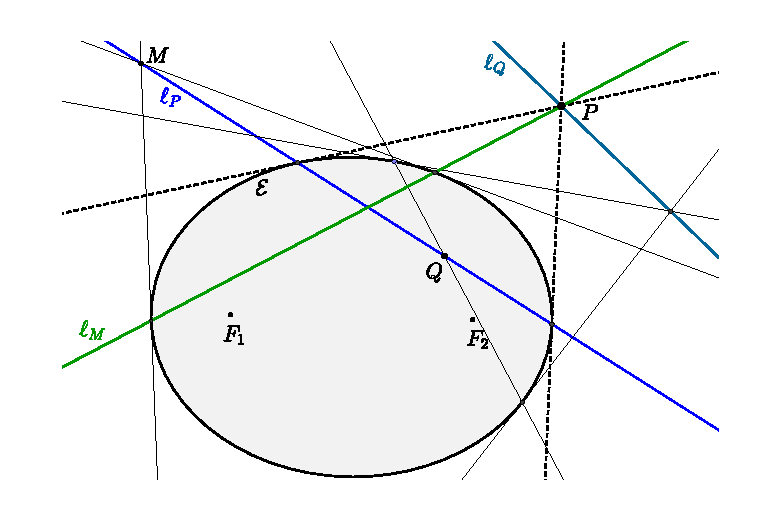
\includegraphics[scale=0.6]{pics_09_003_dual_polarline-pole-elipse.pdf}
    \caption{Duality between pole and polar ($Q \in \ell_P$ and $P\in \ell_Q$).}
    \label{fig:pics-09-polarpole-ellipse}
\end{figure}

\begin{proof} Direct from \cref{lem:09-polarline} and \cref{lem:09-polar}. In fact, let $P=[x_0,y_0]$. Then $\ell_P$ is given by \cref{eqn:09-polarline}. Therefore, if $Q=[x_1,y_1]\in \ell_P$ it follows that
$x_0x_1/a^2+y_0y_1/b^2=1$. This also shows that $P_0\in \ell_Q.$
\end{proof}

\begin{proposition}
    Consider an ellipse $\mathcal{E}$ with foci $F_1$ and $F_2$. Let $\ell_P$ be the tangent line to $\E$ at $P\in \E$. Then $\ell_P$ (also polar line of $P$)  is a bisector of the   lines $PF_1$ and $PF_2$, see \cref{fig:bisectorline}.  
\label{prop:09-bisectorline}
\end{proposition}

\begin{figure} 
	\begin{center}
		 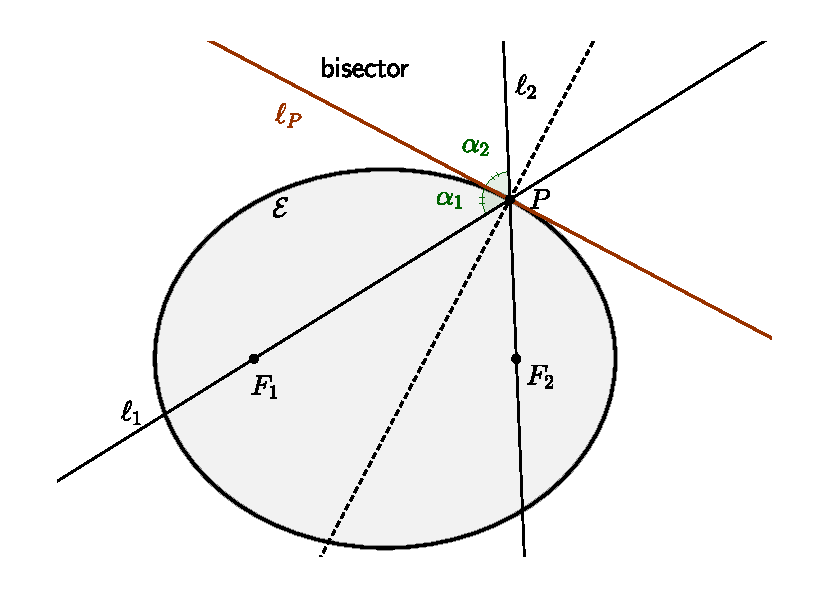
\includegraphics[scale=0.7]{pics_09_001_bisector_tangent_ellipse.pdf}
		\caption {The tangent line $\ell_p$ is a bisector of the external angle, i.e., the angles $\alpha_1$ and $\alpha_2$ are equal. 	\label{fig:bisectorline} }
	\end{center}

\end{figure}

\begin{proof} Let $P=[x_1,y_1]\in \E$. Consider the vectors $V_1=F_1-P$ and $V_2=F_2-P_2$.
Then the external bisector  is parametrized by:  $P+sV_{12}$, where $V_{12}=|V_2|V_1-|V_1|V_2$. As $|V_1|+|V_2|=2a$ for all $P\in \E$ it follows that $N_{12}=V_1/|V_1|+V_2/|V_2|$ is normal to the ellipse. Therefore, $\langle N_{12},V_{12}\rangle=0$. So,
$V_{12}$ is tangent to $\E$.
\end{proof}

Referring to \cref{fig:09-circle-polarline}:

\begin{proposition}
\label{prop:09-circle-polarline}
    Consider an ellipse $\mathcal{E}$ with foci $F_1$ and $F_2$. Let $ P_0 $ be an exterior point and $\ell_{P_0}$ be the polar line associated to $P_0$ intersecting the ellipse $\E$ at $P_1$ and $P_2$. Suppose that $F_2\in \ell_{P_0}$. Then $P_0$ is  the center of a circle $\mathcal{C}_0$  tangent to the polar line line at $F_2$ and to the lines $F_1P_1$ and $F_1P_2$. 
\end{proposition}

\begin{figure} 
	\begin{center}
		 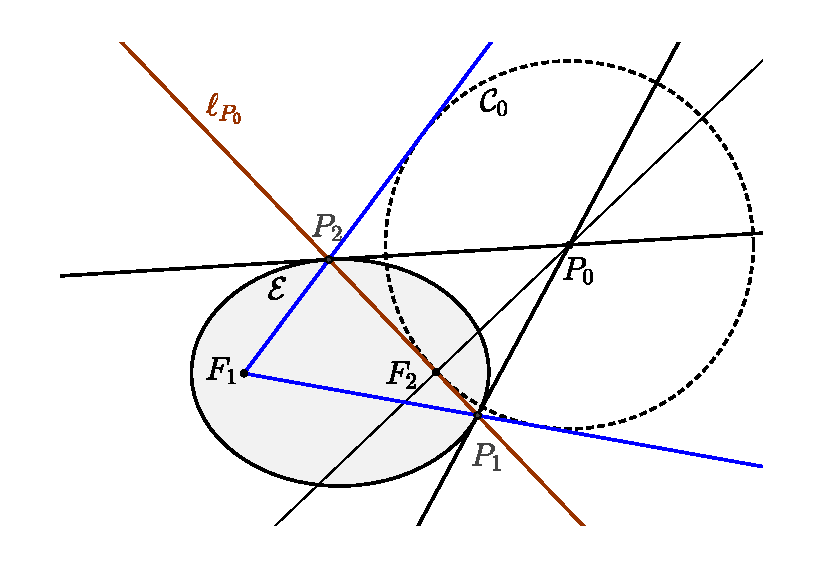
\includegraphics[scale=0.7]{pics_09_002_circle_tangent_polarline.pdf}
		\caption{The polar line $\ell_{P_0}$ passing through the focus $F_2$ is tangent to the excircle $\mathcal{C}_0$ which is centered at $P_0$.}
	\end{center}
\label{fig:09-circle-polarline} 
\end{figure}

\begin{proof}
See \cite[page 10]{akopyan2007-conics}. By \cref{prop:09-bisectorline} the line  $P_0P_2$ (resp. $P_0P_1$) is  the bisector line of $F_1P_2$ and $\ell_{P_0}$ (resp. of $F_1P_1$ and $\ell_{P_0}$). Therefore, there exists a circle $\mathcal{C}_0$ centered at $P_0$ and tangent to $\ell_{P_0}$, $P_1F_1$ and $F_1P_2.$ In fact, $\mathcal{C}_0$ is the excircle of the triangle $F_1P_1P_2$.
Finally we observe that $\ell_{P_0}\cap \mathcal{C}_0$ is $F_2.$ This follows from the property of the excircle $\mathcal{C}_0$ which is tangent to $\ell_{P_0}$ at a point $F_2'$ of the side $P_1P_2$ such that
$ |F_1P_1|+|P_1F_2'|=|P_2F_1| +|P_2F_2'|$. Therefore $F_2=F_2'$, since $F_2$ (focus of $\mathcal{E}$) satisfies the above equation.
\end{proof}
\begin{proposition} Consider an ellipse and two tangent lines passing through an exterior point $P_0$ as shown in   \cref{fig:angulofoco}. Let also the  line passing through the $P_0$ and   focus $F_2$.  Then it follows that that $\alpha_1=\alpha_2$. 
\end{proposition} 

\begin{figure} 
	\begin{center}
  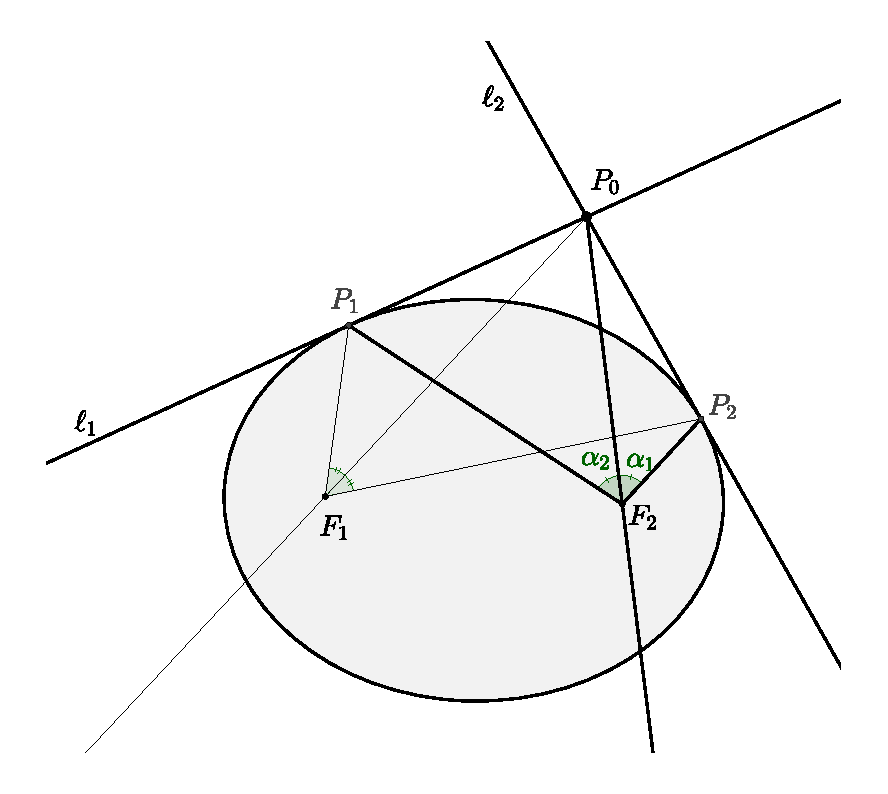
\includegraphics[scale=0.7]{pics_09_050_angulosiguais_foco.pdf}
		\caption {Angles $\alpha_1$ and $\alpha_2$ are equal. 	\label{fig:angulofoco} }
	\end{center}

\end{figure}

\begin{proof} Consider the quadrilateral $F_1P_2F_2P_1.$
Observe that $|F_1P_2|+|P_2F_2|=|F_2P_1|+|P_1F_1|. $
Therefore, there is a circle tangent to the sidelines $F_1P_2$, $F_1P_1$, $F_2P_2$ and $F_2P_1$, which is centered at $P_0.$ So, the line $F_2P_0$ is a bisector of $F_2P_1$ and $F_2P_2.$
\end{proof}



\begin{proposition} Consider an ellipse and two tangent lines passing through an exterior point as shown in    \cref{fig:angulocorda}. Let also the two lines passing through the foci and $P_0$.  Then  we have that $\theta_1=\theta_2$. 
\end{proposition} 

\begin{figure}
	\begin{center}
 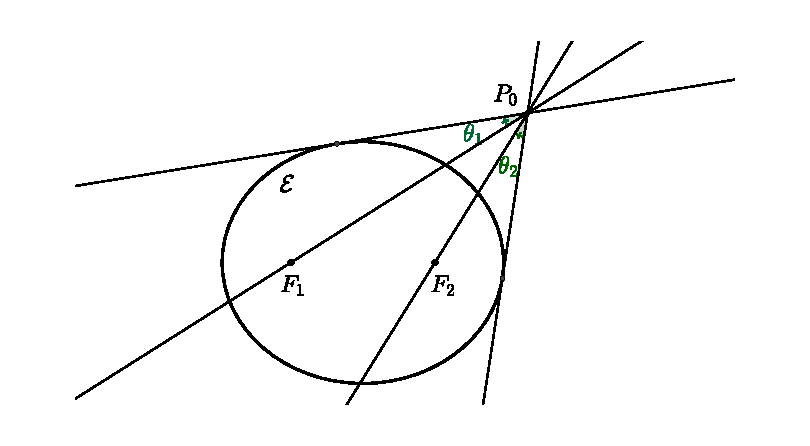
\includegraphics[scale=0.9]{pics_tex/angulo_corda.pdf}
		\caption {Angles $\theta_1$ and $\theta_2$ are equal. 	\label{fig:angulocorda} }
	\end{center}

\end{figure}

 \begin{proof} See \cite{melrose1979} and \cite{akopyan2007-conics}.
Let $O$ be the point of intersection of the lines $F_1P_1$ and $F_2P_2.$
Consider the triangle $P_0F_2P_2$ and the line $F_2Q$ tangent to the circle centered at $P_0.$ See \cref{fig:angulosiguaisproof}.


\begin{figure}
	\begin{center}
 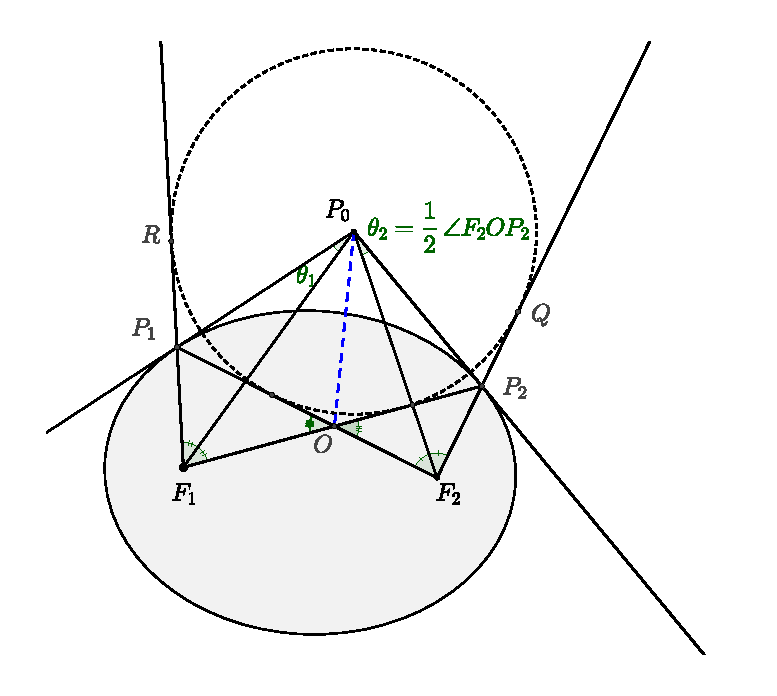
\includegraphics[scale=0.7]{pics_09_040_angulosiguais_proof.pdf}
		\caption {Angle   $\theta_2$ is equal to  $\frac{1}{2}\angle F_2OP_2$.	\label{fig:angulosiguaisproof} }
	\end{center}

\end{figure}

We have that
\begin{align*}
    \theta_2&=\angle F_2P_0P_2=\angle P_0P_2Q-\angle P_0F_2P_2\\ 
    &= \angle P_0P_2Q-\angle P_0F_2P_1\\
    &=\frac{1}{2}\angle F_1P_2Q -\frac{1}{2} \angle P_1F_2Q\\
    &=
    \frac{1}{2} \angle P_2OF_2
 \end{align*}
 The relations above follows from the fact that $P_0F_2$ is a bisector of the lines $P_1F_2$ and $F_2P_2$ and   that  $\angle F_1P_2Q$ is an external angle of triangle $OF_2P_2.$
 Analogously, $\theta_1=\angle P_1OF_1$. So, $\theta_1=\theta_2.$
\end{proof}

\begin{proposition}
	Consider a pair of confocal ellipses $\mathcal{E}$ and $\mathcal{E}'$ with semi-axes $(a,b)$ and $(a_c,b_c)$ respectively. Referring to   \cref{fig:dEE1} it follows that:
	
	\[\frac{|P_0P_1|}{|P_1F_1|}+\frac{|P_0P_2|}{|P_2F_2|}=\frac{2 a_c (a-a_c)}{b_c^2}\]
	is constant (independent of $P_0$).
\label{prop:dEE1}	
\end{proposition}
\begin{figure} 
	\begin{center}	 
  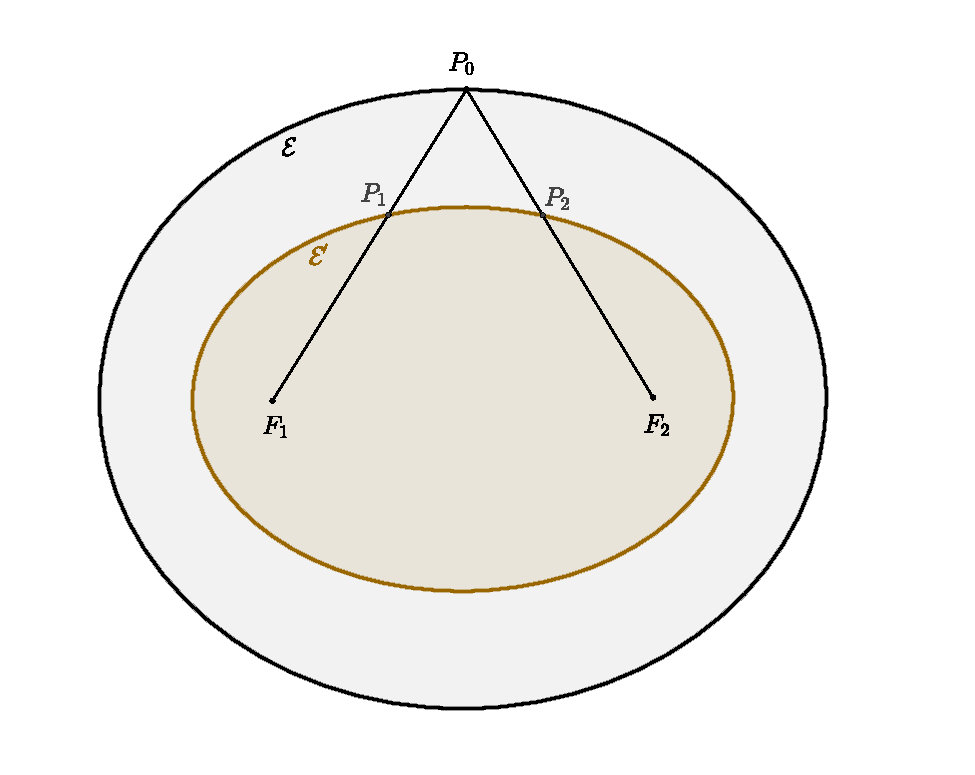
\includegraphics[scale=0.5]{pics_09_060_relacaodEE.pdf}
		\caption { The sum of relation of focal distances is constant. \label{fig:dEE1} }
	\end{center}
	
\end{figure}
\begin{proof} 
Follows from straightforward calculations, computing the quantities involved with help of CAS. 
\end{proof}

\begin{remark} 
The above result is attributed  to   \cite{milena2003} and  \cite{taba2004_magnetic}.  See \cite{akopyan2021}.
\end{remark}

\begin{proposition}
	Consider a confocal pair of an ellipse  $\mathcal{E}$ and a hyperbola $\mathcal{H}$. Referring to   \cref{fig:dEH} it follows that:
	
	\[\frac{|P_0P_1|}{|P_1F_1|}+\frac{|P_0P_2|}{|P_2F_2|}=\frac{2a_c(a+a_c)}{b_c^2}\;\;\; \text{and}\;\;\; \frac{|P_0F_1|}{|P_1'F_1|}+\frac{|P_0F_2|}{|P_2'F_2|}= \frac{2a_c(a-ac)}{b_c^2}\]
	are constant (independent of $P_0$).
 The sums  are constant for $P_0$ in the arc of ellipse  where the points $P_i,\; P'_i$ (i=1,2) are well defined.
\end{proposition}
\begin{figure} 
	\begin{center}
 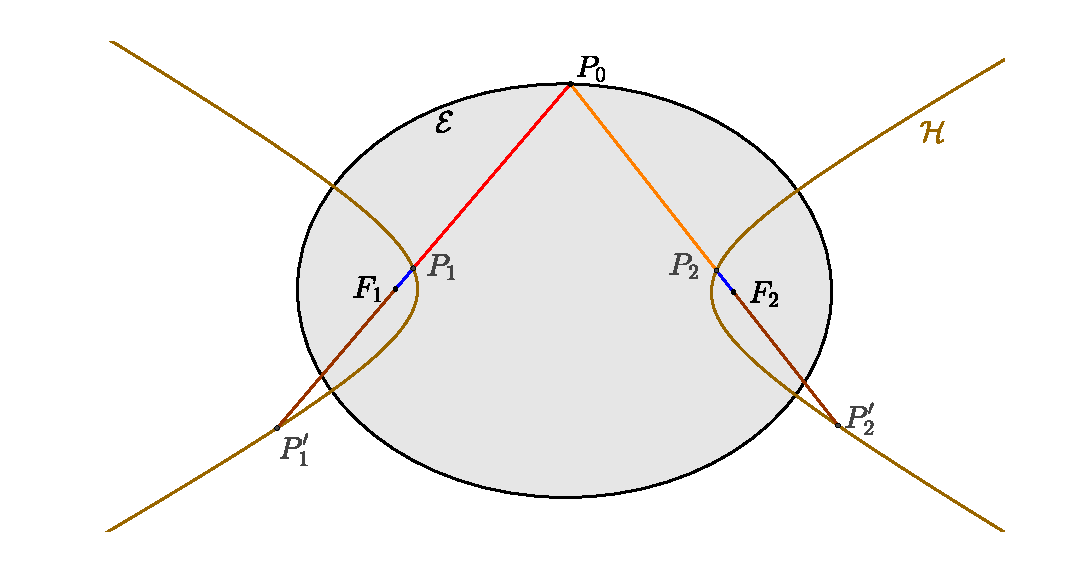
\includegraphics[scale=0.7]{pics_09_070razaoEH_confocal2.pdf}
		\caption { Sum of relations of focal distances in a confocal pair (ellipse and hyperbola) is constant.  }
		\label{fig:dEH}
	\end{center}
\end{figure}
\begin{proof}
Follows from straightforward calculations, computing the quantities involved with help of CAS. 
\end{proof}
\begin{proposition}
	Consider a pair of confocal hyperbolas $\mathcal{H}$ and $\mathcal{H}_1$. Referring to   \cref{fig:dHH} it follows that:
	
	\[\frac{|P_0P_1|}{|P_1F_1|}/\frac{|P_0P_2|}{|P_2F_2|}=\frac{a+a_c}{a-a_c}\]
	is constant (independent of $P_0$).
	
\end{proposition}
\begin{figure}
	\begin{center}
	 %
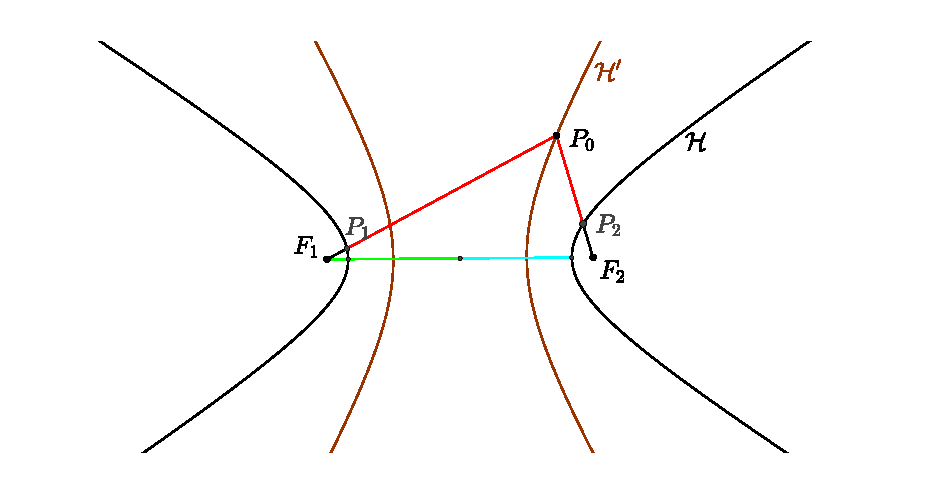
\includegraphics[scale=0.6]{pics_09_080razaoHH1_confocal1.pdf}
		\caption { Relation of focal distances in a pair of confocal hyperbolas. }
		\label{fig:dHH}
	\end{center}
\end{figure}
\begin{proof}
Follows from straightforward calculations, computing the quantities involved with help of CAS. 
\end{proof}


\begin{proposition} \label{prop:pedal_circle} Consider an ellipse $\mathcal{E}$  with foci $F_1=(-c,0)$ and $F_2=(c,0)$. Let $P_0=(x_0,y_0)\in\mathcal{E}$ and $Q_0$ the pedal of $F_2$ with respect to the tangent line passing through $P_0$. Let also $Q_2$ the reflection of $F_2$ with respect to the pedal point $Q_0$.
	Then \[ |Q_2-F_1|=2a\]
	Therefore the locus of points as constructed above is a circle $\mathcal{C}$  of radius $2a$ centered at $F_1$.
	Also the locus of pedal points is a circle centered at the origin and radius $a$.
	
	The pair $\{\mathcal{E},\mathcal{C}\}$ is a Poncelet pair having all periodic orbits of period 3.
\end{proposition}

\begin{figure} 
	\begin{center}
		\def\svgwidth{0.55\textwidth}
		\input{pics_tex/elipse_circulo2a.eps_tex}
		\caption {   }
	\end{center}
	\label{fig:elipse_circulo}
\end{figure}
\begin{proof}


\end{proof}


\begin{theorem}%[ Galperin-Plakhov Theorem]
Consider a pair of confocal conics with foci $F_1$ and $F_2$ in the plane (see   \cref{fig:galperin}).
  Consider  the right branch of the hyperbola associated with $F_2$. Let $P$
and $Q$ be the points of intersection of the ellipse with the right branch of the hyperbola.
Consider a ray starting at $F_1$ and intersecting the right branch of the hyperbola. Denote
by $B$ (resp.\ $A$ ) the intersection points of this ray with the ellipse (resp.\  with the right branch of the
hyperbola). Suppose the focus $F_2$ lies on the line $P Q$. Then the line $P Q$ is the bisector of the
angle $  \angle  AF_2B$.  
\end{theorem}
\begin{figure} 
	\begin{center}
		\def\svgwidth{0.75\textwidth}
 	\input{pics_tex/galperin.eps_tex}
	 %	 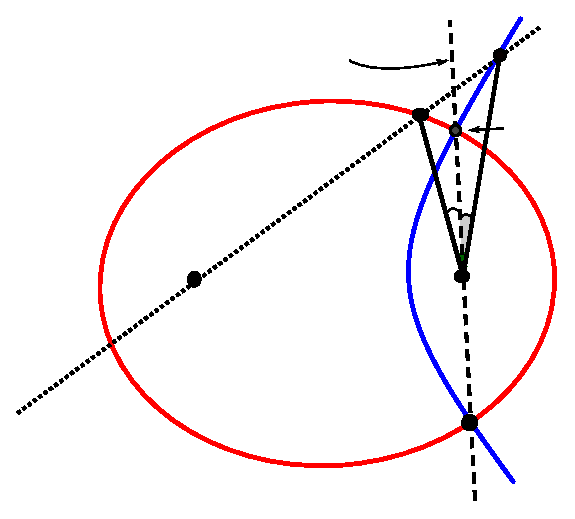
\includegraphics[angle=0, width=10cm]{pics_tex/galperin.eps}
		\caption { The line $PQ$ passing through the focus $F_2$ and the intersection of the ellipse with the right branch of the hyperbola  is a bisector of the angle $AF_2B$.}
		 \label{fig:galperin}
	\end{center}
\end{figure}
\begin{proof}
See \cite{dolgirev2014} for a synthetic proof.
Considering the parametrization of the confocal family  of conics it follows that
\begin{align*}
    A&=[c\cos u\cosh v,c \sin u \sinh v]\\
    B&=\left[ {\frac {2c{{\rm e}^{v}}}{\cos u \left( {
{\rm e}^{2\,v}}+1 \right) }},{\frac { c \left( {{\rm e}^{2\,v}}-1
 \right) \sin u  }{\cos u
 \left( {{\rm e}^{2\,v}}+1 \right) }}\right]\\
    P&=[c,c\sin u\tan u],\;\;Q=[c,-c\sin u\tan u].  
\end{align*}
Performing the calculations it follows that
\[\cos(\angle PF_2A)=\cos(\angle PF_2B)\]
\end{proof}

\begin{theorem}\label{th:ehfocus}
Consider a pair of confocal conics (ellipse and hyperbola). Let $M$ be  an arbitrary point $M$ (exterior to the ellipse)
on the line passing through the intersection points $P$ and $Q$ of the ellipse and the right branch of
the hyperbola. Draw two tangent lines to the ellipse and to the hyperbola. Then the   lines $P_1Q_1$ and $P_2Q_2$ (resp.\ $P_1Q_2$ and $P_2Q_1$)
through the tangent points as shown in \cref{fig:ehfocus}  passe  through the focus $F_1$ (resp.\   $F_2$). 
\end{theorem}


\begin{figure}
	\begin{center}
 	 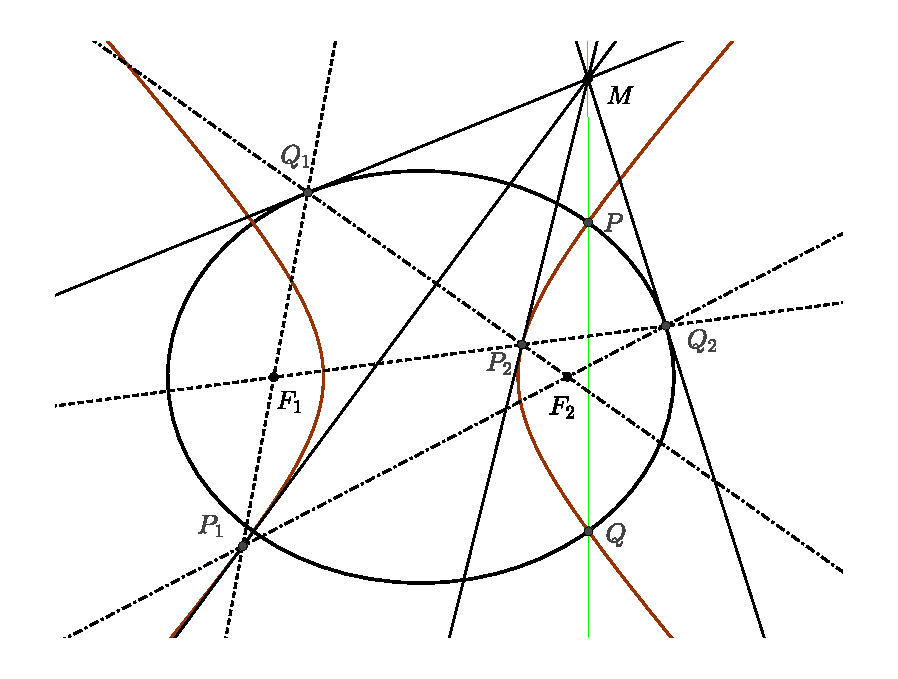
\includegraphics[scale=0.6]{pics_09_090_elipse_hiperbole_focus1.pdf}
		\caption{The four lines passing through the point $M$ and tangent to the confocal conics determine four lines passing through the foci. \label{fig:ehfocus}}
	\end{center}
\end{figure}
\begin{proof}
See \cite{dolgirev2014}. A direct proof can be performed computing the intersection points $\{P_1,P_2\}$ (resp.\ $\{Q_1,Q_2\}$) of the tangent lines passing through $M$ with the hyperbola (resp.\ ellipse). After this, it is straightforward to obtain that $F_1= Q_1P_1\cap P_2Q2$
and $F_2= Q_2P_1\cap Q_1Q2$. 
In the above analysis the property of of $M$ being in the straight line $PQ$ and that the pair of conics are confocal is essential.
\end{proof}
\begin{remark}
The pair of tangent lines to a hyperbola $x^2/a^2-y^2/b^2=1$ and passing through $M=(x_0,y_0)$ is given by
\[ b^2(x - x_0)^2 -a^2(y - y_0)^2  + (xy_0 - x_0y)^2=0.
\]
\end{remark}

 \begin{theorem}\label{th:dolgirev}
 Let two confocal ellipses $\E_1$ and $\E_2$   with foci $F_1 $ and $F_2$ are given. Let a
 ray with the origin at $F_1$ intersects $\E_1$ and $\E_2$ at $A$ and $B$, respectively. Let a ray with
 the origin at $F_2$ intersects $\E_1$ and $\E_2$ at $C$ and $D$, respectively. Suppose the points $B$ and
 $C$ lie on a branch $\mathcal{H}_1$   of the hyperbola with the foci at $F_1$ and $F_2$.
 Then the points $A$
 and $D$ lie on a branch $\mathcal{H}_2$ of the confocal hyperbola with the foci at $F_1$ and $F_2$. (see \cref{fig:retangulo_EH})

 %\noindent b) Consider a ray starting at $F_1$ intersecting the branch $\mathcal{H}_1$ at $P_1$. Consider the ray
 %$F_2P_1$  intersecting the ellipse $\E_2$  at $P_2$. Analogously, we define the points $P_3$, $P_4$, $P_5$.
% Then $P_5=P_1.$
 \end{theorem}

 \begin{figure} 
 	\begin{center}
 	 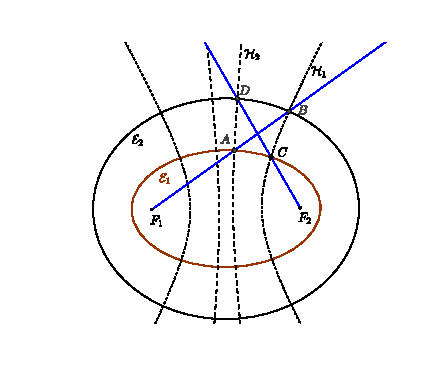
\includegraphics[scale=1]{pics_09_100_confocal_retangulo.pdf}
 		\caption {Quadrangle $ACBD$ with vertices and diagonal  $AB$ (resp.\ $CD$) passing through $F_1$ (resp.\   $F_2$).
 		 \label{fig:retangulo_EH} }
 	\end{center}

 \end{figure}

 \begin{proof}
 See \cite{dolgirev2014}.
\end{proof}

 